\documentclass[../main/NEMO_manual]{subfiles}

\begin{document}
% ================================================================
% Chapter 1 Model Basics
% ================================================================
% ================================================================
% Curvilinear \zstar- \sstar-coordinate System
% ================================================================
\chapter{ essai \zstar \sstar}
\section{Curvilinear \zstar- or \sstar coordinate system}

% -------------------------------------------------------------------------------------------------------------
% ????
% -------------------------------------------------------------------------------------------------------------

\colorbox{yellow}{ to be updated }

In that case, the free surface equation is nonlinear, and the variations of volume are fully taken into account.
These coordinates systems is presented in a report \citep{Levier2007} available on the \NEMO web site. 

\colorbox{yellow}{  end of to be updated}

% from MOM4p1 documentation

To overcome problems with vanishing surface and/or bottom cells, we consider the zstar coordinate 
\[
  % \label{eq:PE_}
  z^\star = H \left( \frac{z-\eta}{H+\eta} \right)
\]

This coordinate is closely related to the "eta" coordinate used in many atmospheric models
(see Black (1994) for a review of eta coordinate atmospheric models).
It was originally used in ocean models by Stacey et al. (1995) for studies of tides next to shelves,
and it has been recently promoted by Adcroft and Campin (2004) for global climate modelling.

The surfaces of constant $z^\star$ are quasi-horizontal.
Indeed, the $z^\star$ coordinate reduces to $z$ when $\eta$ is zero.
In general, when noting the large differences between undulations of the bottom topography versus undulations in
the surface height, it is clear that surfaces constant $z^\star$ are very similar to the depth surfaces.
These properties greatly reduce difficulties of computing the horizontal pressure gradient relative to
terrain following sigma models discussed in \autoref{subsec:PE_sco}. 
Additionally, since $z^\star$ when $\eta = 0$, no flow is spontaneously generated in
an unforced ocean starting from rest, regardless the bottom topography.
This behaviour is in contrast to the case with "s"-models, where pressure gradient errors in the presence of
nontrivial topographic variations can generate nontrivial spontaneous flow from a resting state,
depending on the sophistication of the pressure gradient solver.
The quasi-horizontal nature of the coordinate surfaces also facilitates the implementation of
neutral physics parameterizations in $z^\star$ models using the same techniques as in $z$-models
(see Chapters 13-16 of Griffies (2004) for a discussion of neutral physics in $z$-models,
as well as  \autoref{sec:LDF_slp} in this document for treatment in \NEMO). 

The range over which $z^\star$ varies is time independent $-H \leq z^\star \leq 0$.
Hence, all cells remain nonvanishing, so long as the surface height maintains $\eta > ?H$.
This is a minor constraint relative to that encountered on the surface height when using $s = z$ or $s = z - \eta$. 

Because $z^\star$ has a time independent range, all grid cells have static increments ds,
and the sum of the ver tical increments yields the time independent ocean depth %�k ds = H. 
The $z^\star$ coordinate is therefore invisible to undulations of the free surface,
since it moves along with the free surface.
This proper ty means that no spurious ver tical transpor t is induced across surfaces of
constant $z^\star$ by the motion of external gravity waves.
Such spurious transpor t can be a problem in z-models, especially those with tidal forcing.
Quite generally, the time independent range for the $z^\star$ coordinate is a very convenient property that
allows for a nearly arbitrary vertical resolution even in the presence of large amplitude fluctuations of
the surface height, again so long as $\eta > -H$. 

%%%
%  essai update time splitting...
%%%

% ================================================================
% Surface Pressure Gradient and Sea Surface Height
% ================================================================
\section{Surface pressure gradient and sea surface heigth (\protect\mdl{dynspg})}
\label{sec:DYN_hpg_spg}
%-----------------------------------------nam_dynspg----------------------------------------------------

%\nlst{nam_dynspg} 
%------------------------------------------------------------------------------------------------------------
Options are defined through the \ngn{nam\_dynspg} namelist variables.
The surface pressure gradient term is related to the representation of the free surface (\autoref{sec:PE_hor_pg}).
The main distinction is between the fixed volume case (linear free surface or rigid lid) and
the variable volume case (nonlinear free surface, \key{vvl} is active).
In the linear free surface case (\autoref{subsec:PE_free_surface}) and rigid lid (\autoref{PE_rigid_lid}),
the vertical scale factors $e_{3}$ are fixed in time,
while in the nonlinear case (\autoref{subsec:PE_free_surface}) they are time-dependent.
With both linear and nonlinear free surface, external gravity waves are allowed in the equations,
which imposes a very small time step when an explicit time stepping is used.
Two methods are proposed to allow a longer time step for the three-dimensional equations:
the filtered free surface, which is a modification of the continuous equations %(see \autoref{eq:PE_flt}),
and the split-explicit free surface described below.
The extra term introduced in the filtered method is calculated implicitly,
so that the update of the next velocities is done in module \mdl{dynspg\_flt} and not in \mdl{dynnxt}.

%-------------------------------------------------------------
% Explicit
%-------------------------------------------------------------
\subsubsection{Explicit (\protect\key{dynspg\_exp})}
\label{subsec:DYN_spg_exp}

In the explicit free surface formulation, the model time step is chosen small enough to
describe the external gravity waves (typically a few ten seconds).
The sea surface height is given by:
\begin{equation}
  \label{eq:dynspg_ssh}
  \frac{\partial \eta }{\partial t}\equiv \frac{\text{EMP}}{\rho_w }+\frac{1}{e_{1T}
    e_{2T} }\sum\limits_k {\left( {\delta_i \left[ {e_{2u} e_{3u} u}
        \right]+\delta_j \left[ {e_{1v} e_{3v} v} \right]} \right)}
\end{equation}

where EMP is the surface freshwater budget (evaporation minus precipitation, and minus river runoffs
(if the later are introduced as a surface freshwater flux, see \autoref{chap:SBC}) expressed in $Kg.m^{-2}.s^{-1}$,
and $\rho_w =1,000\,Kg.m^{-3}$ is the volumic mass of pure water.
The sea-surface height is evaluated using a leapfrog scheme in combination with an Asselin time filter,
(\ie the velocity appearing in (\autoref{eq:dynspg_ssh}) is centred in time (\textit{now} velocity). 

The surface pressure gradient, also evaluated using a leap-frog scheme, is then simply given by:
\begin{equation}
  \label{eq:dynspg_exp}
  \left\{
    \begin{aligned}
      - \frac{1}    						{e_{1u}} \;	\delta_{i+1/2} \left[  \,\eta\,  \right] \\ \\
      - \frac{1}    						{e_{2v}} \;	\delta_{j+1/2} \left[  \,\eta\,  \right]
    \end{aligned}
  \right.
\end{equation} 

Consistent with the linearization, a $\left. \rho \right|_{k=1} / \rho_o$ factor is omitted in
(\autoref{eq:dynspg_exp}). 

%-------------------------------------------------------------
% Split-explicit time-stepping
%-------------------------------------------------------------
\subsubsection{Split-explicit time-stepping (\protect\key{dynspg\_ts})}
\label{subsec:DYN_spg_ts}
%--------------------------------------------namdom----------------------------------------------------

\nlst{namdom} 
%--------------------------------------------------------------------------------------------------------------
The split-explicit free surface formulation used in OPA follows the one proposed by \citet{Griffies2004}.
The general idea is to solve the free surface equation with a small time step,
while the three dimensional prognostic variables are solved with a longer time step that
is a multiple of \np{rdtbt} in the \ngn{namdom} namelist (Figure III.3). 

%>   >   >   >   >   >   >   >   >   >   >   >   >   >   >   >   >   >   >   >   >   >   >   >   >   >   >   >
\begin{figure}[!t]
  \begin{center}
    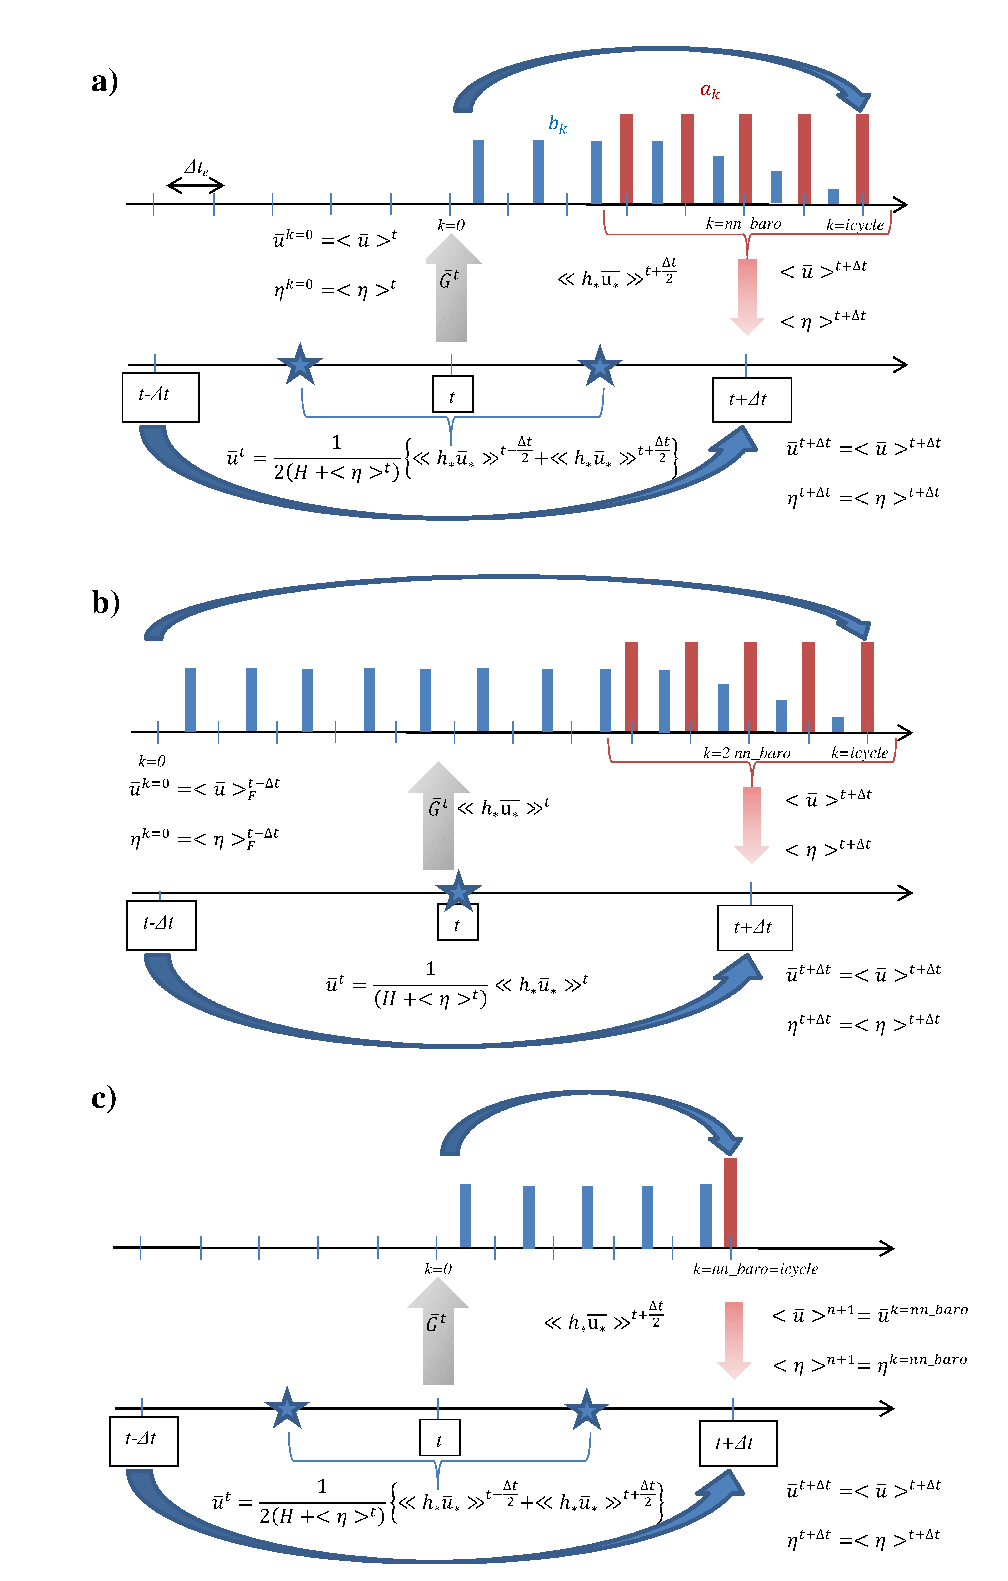
\includegraphics[width=0.90\textwidth]{Fig_DYN_dynspg_ts}
    \caption{
      \protect\label{fig:DYN_dynspg_ts}
      Schematic of the split-explicit time stepping scheme for the barotropic and baroclinic modes,
      after \citet{Griffies2004}.
      Time increases to the right.
      Baroclinic time steps are denoted by $t-\Delta t$, $t, t+\Delta t$, and $t+2\Delta t$.
      The curved line represents a leap-frog time step,
      and the smaller barotropic time steps $N \Delta t=2\Delta t$ are denoted by the zig-zag line.
      The vertically integrated forcing \textbf{M}(t) computed at
      baroclinic time step t represents the interaction between the barotropic and baroclinic motions.
      While keeping the total depth, tracer, and freshwater forcing fields fixed,
      a leap-frog integration carries the surface height and vertically integrated velocity from
      t to $t+2 \Delta t$ using N barotropic time steps of length $\Delta t$.
      Time averaging the barotropic fields over the N+1 time steps (endpoints included)
      centers the vertically integrated velocity at the baroclinic timestep $t+\Delta t$.
      A baroclinic leap-frog time step carries the surface height to $t+\Delta t$ using the convergence of
      the time averaged vertically integrated velocity taken from baroclinic time step t.
    }
  \end{center}
\end{figure}
%>   >   >   >   >   >   >   >   >   >   >   >   >   >   >   >   >   >   >   >   >   >   >   >   >   >   >   >

The split-explicit formulation has a damping effect on external gravity waves,
which is weaker than the filtered free surface but still significant as shown by \citet{Levier2007} in
the case of an analytical barotropic Kelvin wave. 

%from griffies book: .....   copy past !

\textbf{title: Time stepping the barotropic system }

Assume knowledge of the full velocity and tracer fields at baroclinic time $\tau$.
Hence, we can update the surface height and vertically integrated velocity with a leap-frog scheme using
the small barotropic time step $\Delta t$.
We have
\[
  % \label{eq:DYN_spg_ts_eta}
  \eta^{(b)}(\tau,t_{n+1}) - \eta^{(b)}(\tau,t_{n+1}) (\tau,t_{n-1})
  = 2 \Delta t \left[-\nabla \cdot \textbf{U}^{(b)}(\tau,t_n) + \text{EMP}_w(\tau) \right] 
\]
\begin{multline*}
  % \label{eq:DYN_spg_ts_u}
  \textbf{U}^{(b)}(\tau,t_{n+1}) - \textbf{U}^{(b)}(\tau,t_{n-1})  \\
  = 2\Delta t \left[ - f \textbf{k} \times \textbf{U}^{(b)}(\tau,t_{n})
    - H(\tau) \nabla p_s^{(b)}(\tau,t_{n}) +\textbf{M}(\tau) \right]
\end{multline*}
\

In these equations, araised (b) denotes values of surface height and
vertically integrated velocity updated with the barotropic time steps.
The $\tau$ time label on $\eta^{(b)}$ and $U^{(b)}$ denotes the baroclinic time at which
the vertically integrated forcing $\textbf{M}(\tau)$
(note that this forcing includes the surface freshwater forcing), the tracer fields,
the freshwater flux $\text{EMP}_w(\tau)$, and total depth of the ocean $H(\tau)$ are held for
the duration of the barotropic time stepping over a single cycle.
This is also the time that sets the barotropic time steps via 
\[
  % \label{eq:DYN_spg_ts_t}
  t_n=\tau+n\Delta t   
\]
with $n$ an integer.
The density scaled surface pressure is evaluated via 
\[
  % \label{eq:DYN_spg_ts_ps}
  p_s^{(b)}(\tau,t_{n}) =
  \begin{cases}
    g \;\eta_s^{(b)}(\tau,t_{n}) \;\rho(\tau)_{k=1}) / \rho_o  &      \text{non-linear case} \\
    g \;\eta_s^{(b)}(\tau,t_{n})  &      \text{linear case}
  \end{cases}
\]
To get started, we assume the following initial conditions 
\[
  % \label{eq:DYN_spg_ts_eta}
  \begin{split}
    \eta^{(b)}(\tau,t_{n=0}) &= \overline{\eta^{(b)}(\tau)} \\
    \eta^{(b)}(\tau,t_{n=1}) &= \eta^{(b)}(\tau,t_{n=0}) + \Delta t \ \text{RHS}_{n=0}
  \end{split}
\]
with 
\[
  % \label{eq:DYN_spg_ts_etaF}
  \overline{\eta^{(b)}(\tau)} = \frac{1}{N+1} \sum\limits_{n=0}^N \eta^{(b)}(\tau-\Delta t,t_{n})
\]
the time averaged surface height taken from the previous barotropic cycle.
Likewise,
\[
  % \label{eq:DYN_spg_ts_u}
  \textbf{U}^{(b)}(\tau,t_{n=0}) = \overline{\textbf{U}^{(b)}(\tau)}	\\ \\
  \textbf{U}(\tau,t_{n=1}) = \textbf{U}^{(b)}(\tau,t_{n=0}) + \Delta t \ \text{RHS}_{n=0}
\]
with 
\[
  % \label{eq:DYN_spg_ts_u}
  \overline{\textbf{U}^{(b)}(\tau)} = \frac{1}{N+1} \sum\limits_{n=0}^N\textbf{U}^{(b)}(\tau-\Delta t,t_{n})
\]
the time averaged vertically integrated transport.
Notably, there is no Robert-Asselin time filter used in the barotropic portion of the integration. 

Upon reaching $t_{n=N} = \tau + 2\Delta \tau$ , the vertically integrated velocity is time averaged to
produce the updated vertically integrated velocity at baroclinic time $\tau + \Delta \tau$ 
\[
  % \label{eq:DYN_spg_ts_u}
  \textbf{U}(\tau+\Delta t) = \overline{\textbf{U}^{(b)}(\tau+\Delta t)}
  = \frac{1}{N+1} \sum\limits_{n=0}^N\textbf{U}^{(b)}(\tau,t_{n})
\]
The surface height on the new baroclinic time step is then determined via
a baroclinic leap-frog using the following form 
\begin{equation}
  \label{eq:DYN_spg_ts_ssh}
  \eta(\tau+\Delta) - \eta^{F}(\tau-\Delta) = 2\Delta t \ \left[ - \nabla \cdot \textbf{U}(\tau) + \text{EMP}_w \right]
\end{equation}

The use of this "big-leap-frog" scheme for the surface height ensures compatibility between
the mass/volume budgets and the tracer budgets.
More discussion of this point is provided in Chapter 10 (see in particular Section 10.2). 
 
In general, some form of time filter is needed to maintain integrity of the surface height field due to
the leap-frog splitting mode in equation \autoref{eq:DYN_spg_ts_ssh}.
We have tried various forms of such filtering,
with the following method discussed in Griffies et al. (2001) chosen due to its stability and
reasonably good maintenance of tracer conservation properties (see ??) 

\begin{equation}
  \label{eq:DYN_spg_ts_sshf}
  \eta^{F}(\tau-\Delta) =  \overline{\eta^{(b)}(\tau)}
\end{equation}
Another approach tried was 

\[
  % \label{eq:DYN_spg_ts_sshf2}
  \eta^{F}(\tau-\Delta) = \eta(\tau)
  + (\alpha/2) \left[\overline{\eta^{(b)}}(\tau+\Delta t)
    + \overline{\eta^{(b)}}(\tau-\Delta t) -2 \;\eta(\tau) \right]
\]

which is useful since it isolates all the time filtering aspects into the term multiplied by $\alpha$.
This isolation allows for an easy check that tracer conservation is exact when eliminating tracer and
surface height time filtering (see ?? for more complete discussion).
However, in the general case with a non-zero $\alpha$, the filter \autoref{eq:DYN_spg_ts_sshf} was found to
be more conservative, and so is recommended. 

%-------------------------------------------------------------
% Filtered formulation 
%-------------------------------------------------------------
\subsubsection{Filtered formulation (\protect\key{dynspg\_flt})}
\label{subsec:DYN_spg_flt}

The filtered formulation follows the \citet{Roullet2000} implementation.
The extra term introduced in the equations (see {\S}I.2.2) is solved implicitly.
The elliptic solvers available in the code are documented in \autoref{chap:MISC}.
The amplitude of the extra term is given by the namelist variable \np{rnu}.
The default value is 1, as recommended by \citet{Roullet2000}

\colorbox{red}{\np{rnu}\forcode{ = 1} to be suppressed from namelist !}

%-------------------------------------------------------------
% Non-linear free surface formulation 
%-------------------------------------------------------------
\subsection{Non-linear free surface formulation (\protect\key{vvl})}
\label{subsec:DYN_spg_vvl}

In the non-linear free surface formulation, the variations of volume are fully taken into account.
This option is presented in a report \citep{Levier2007} available on the NEMO web site.
The three time-stepping methods (explicit, split-explicit and filtered) are the same as in
\autoref{DYN_spg_linear} except that the ocean depth is now time-dependent.
In particular, this means that in filtered case, the matrix to be inverted has to be recomputed at each time-step.

\biblio

\pindex

\end{document}
